\documentclass[a4paper,15pt]{article} % Choose article class with A4 size and 15pt font
% Language setting
% Replace `english' with e.g. `spanish' to change the document language
\usepackage[english]{babel}

% Set page size and margins
% Replace `letterpaper' with `a4paper' for UK/EU standard size
\usepackage[letterpaper,top=2cm,bottom=2cm,left=3cm,right=3cm,marginparwidth=1.75cm]{geometry}

% Useful packages
\usepackage{amsmath}
\usepackage{amssymb} % For additional math symbols
\usepackage{graphicx} % For including graphics (if needed later)
\usepackage[colorlinks=true, allcolors=blue]{hyperref} % For hyperlinks in the document

% Define a custom keywords command:
\providecommand{\keywords}[1]{\textbf{Keywords:} #1}

\title{Analytical Sensitivity Analysis for 1D Thermal Diffusion Model}
\author{Lazizbek Sadullaev}

\begin{document}
\maketitle

\begin{abstract}
Analytical sensitivity analysis for one-dimensional (1D) thermal diffusion models provides a powerful approach to understanding how changes in input parameters affect system behavior. This study focuses on local sensitivity analysis, investigating the cooling rates of spatter deposits modeled using a 1D thermal diffusion equation. By examining small perturbations in thermal diffusivity, the analysis establishes direct relationships between material properties and cooling rates. These findings offer insights into environmental factors affecting thermal processes, contribute to the optimization of thermal management in engineering applications, and improve predictive modeling in material science.
\end{abstract}

% Include keywords
\noindent\textbf{Keywords:} local sensitivity analysis, thermal diffusion, heat equation, parameter sensitivity, material properties, thermal diffusivity, cooling rates, analytical modeling, spatter deposits.

\section{Introduction}

Understanding the sensitivity of mathematical models is crucial in many fields of science and engineering. Numerous studies have been conducted to predict the cooling rates of spatter deposits, aiming to enhance our understanding of these systems. For example, previous work by Claire Elizabeth and Sergey Lapin (2021) investigated the influence of changing material properties (specifically the size of clasts in a volcanic process) on the cooling time of spatter piles \cite{puleio_project}.

In one of the simpler cases of their work (Model 1), the cooling condition of spatter deposits was modeled as a one-dimensional system, considering a single clast with variable material properties cooling by conduction. Claire Elizabeth explored heat transfer in this system using numerical methods such as finite difference and finite element techniques.

For the model (Fig. 1A, B, p.18), the ground is assumed to be basalt with an initial temperature of 293 K. The clast, also basalt, starts at an initial temperature of either 1073 K or 1373 K, while the air temperature is 293 K. This setup implies that the initial function \( f(x) \) is a step function. Neumann boundary conditions (prescribed heat flux) are applied at the ground/air, ground/clast, clast/clast, and clast/air boundaries, while Dirichlet boundary conditions (fixed temperature) are enforced along the system's exterior boundaries. General schematics of the models are provided in Figures 1 and 2 (p.17).

This problem can then be described by the 1D heat diffusion equation as follows (derivation reference: \href{https://ocw.mit.edu/courses/18-303-linear-partial-differential-equations-fall-2006/d11b374a85c3fde55ec971fe587f8a50_heateqni.pdf}{MIT’s PDE Class}):

\begin{equation}
    \frac{\partial T}{\partial t} = \kappa \frac{\partial^2 T}{\partial x^2}, \quad 0 < x < L, \; t > 0,
    \label{eq:Heat_Equation}
\end{equation}
with initial and boundary conditions:
\begin{align}
    \text{IC:} \; & T(x,0) = f(x), \; 0 < x < L, \label{eq:Initial_Condition} \\
    \text{BC:} \; & T(0,t) = T(L,t) = 0, \; t > 0. \label{eq:Dirichlet_Boundary_Condition}
\end{align}

Here, \( T(x,t) \) represents the temperature at position \( x \) and time \( t \), \( \kappa \) is the thermal diffusivity, and \( f(x) \) defines the initial temperature distribution.

This paper focuses on local sensitivity analysis of the 1D heat diffusion model, aiming to understand how small perturbations in thermal diffusivity \( \kappa \) affect the temperature distribution. Such analysis provides valuable insights into the relationship between material properties and thermal behavior, which are critical in applications ranging from material science to environmental engineering.

This study is motivated by the need for precise modeling and robust predictions in systems where thermal diffusivity varies due to external factors or material heterogeneity. For instance, understanding these effects can improve the design of heat-resistant materials or optimize thermal management systems in engineering applications.

The scope of this work is outlined as follows: In the next section, we provide background material on sensitivity analysis and the heat equation. Following this, we derive the sensitivity equations and discuss their solutions. Additionally, comparisons are made with numerical results from Claire Elizabeth's work to validate our analytical approach. Specific examples are analyzed to illustrate the impact of parameter changes. Finally, the study concludes with a summary of findings and reflections on their broader implications.

\begin{figure}[h!]
\centering
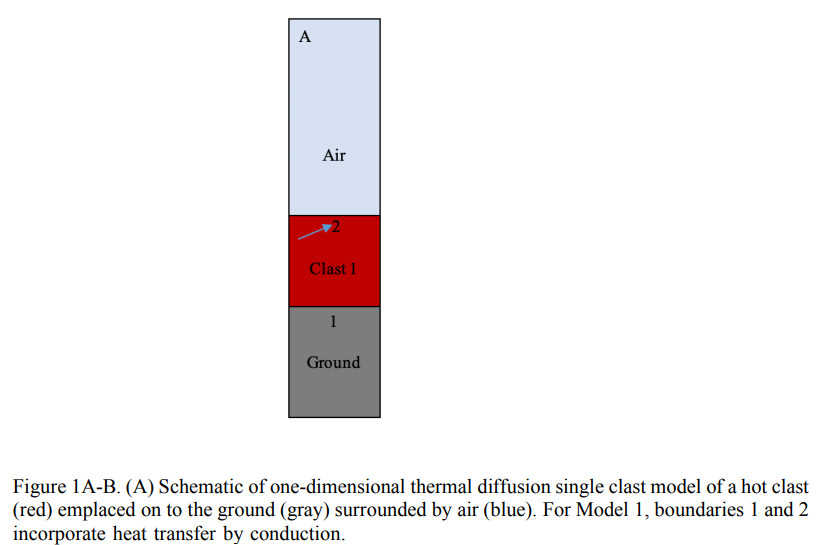
\includegraphics[width=1\linewidth]{intruducing_project.jpg}
\caption{\label{Introducing_project} Explanation of the origin of the model.}
\end{figure}
\newpage


\end{document}
